The User Interface consists in a single page application, divided into three main views: the \textit{Request}, \textit{Response} and \textit{Map view}, as proposed in section \ref{sec:csa_design} and illustrated in figure \ref{fig:csa_tree}. Since the application is developed using React, every view is managed by a container, which reads the state from the store, calls the rendering of presentational components, and may dispatch actions on user input or other events. 

\begin{figure}[htpb]
  \centering
  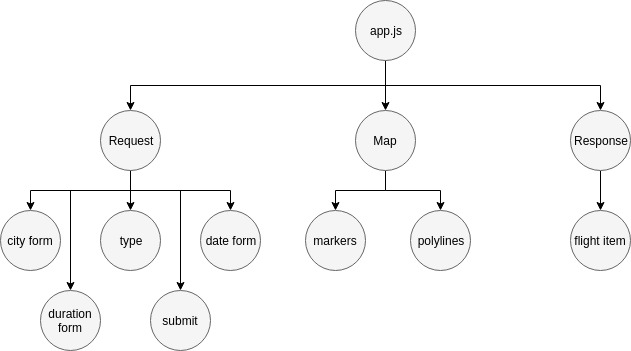
\includegraphics[width=.8\textwidth]{./Figures/system_implementation/csa_tree.jpg}
  \caption{Structure of the developed user interface}
  \label{fig:csa_tre}  
\end{figure}

The User Interface is designed to be mobile friendly, by being responsive to the device size. This is achieved using the Bootstrap grid system, a web application design paradigm in which the user screen is divided into 12 columns, and each element of the user interface may specify a variable number of columns, depending on the screen size.

Figure \ref{fig:desktop_app} and \ref{fig:mobile_app} illustrate two possible views of the developed application. The first image illustrates the application in a desktop device and the second in a mobile. It is worth noting that these two screenshots correspond to the same application, and that the design differences between both images are a result of the responsiveness of the application. The responsive design is responsible for resizing the application elements according to the device size and also includes toggles in the \textit{Request} and \textit{Response} views, as to generate more space to the map view. 


\begin{figure}
\centering
\begin{minipage}{.7\textwidth}
  \centering
  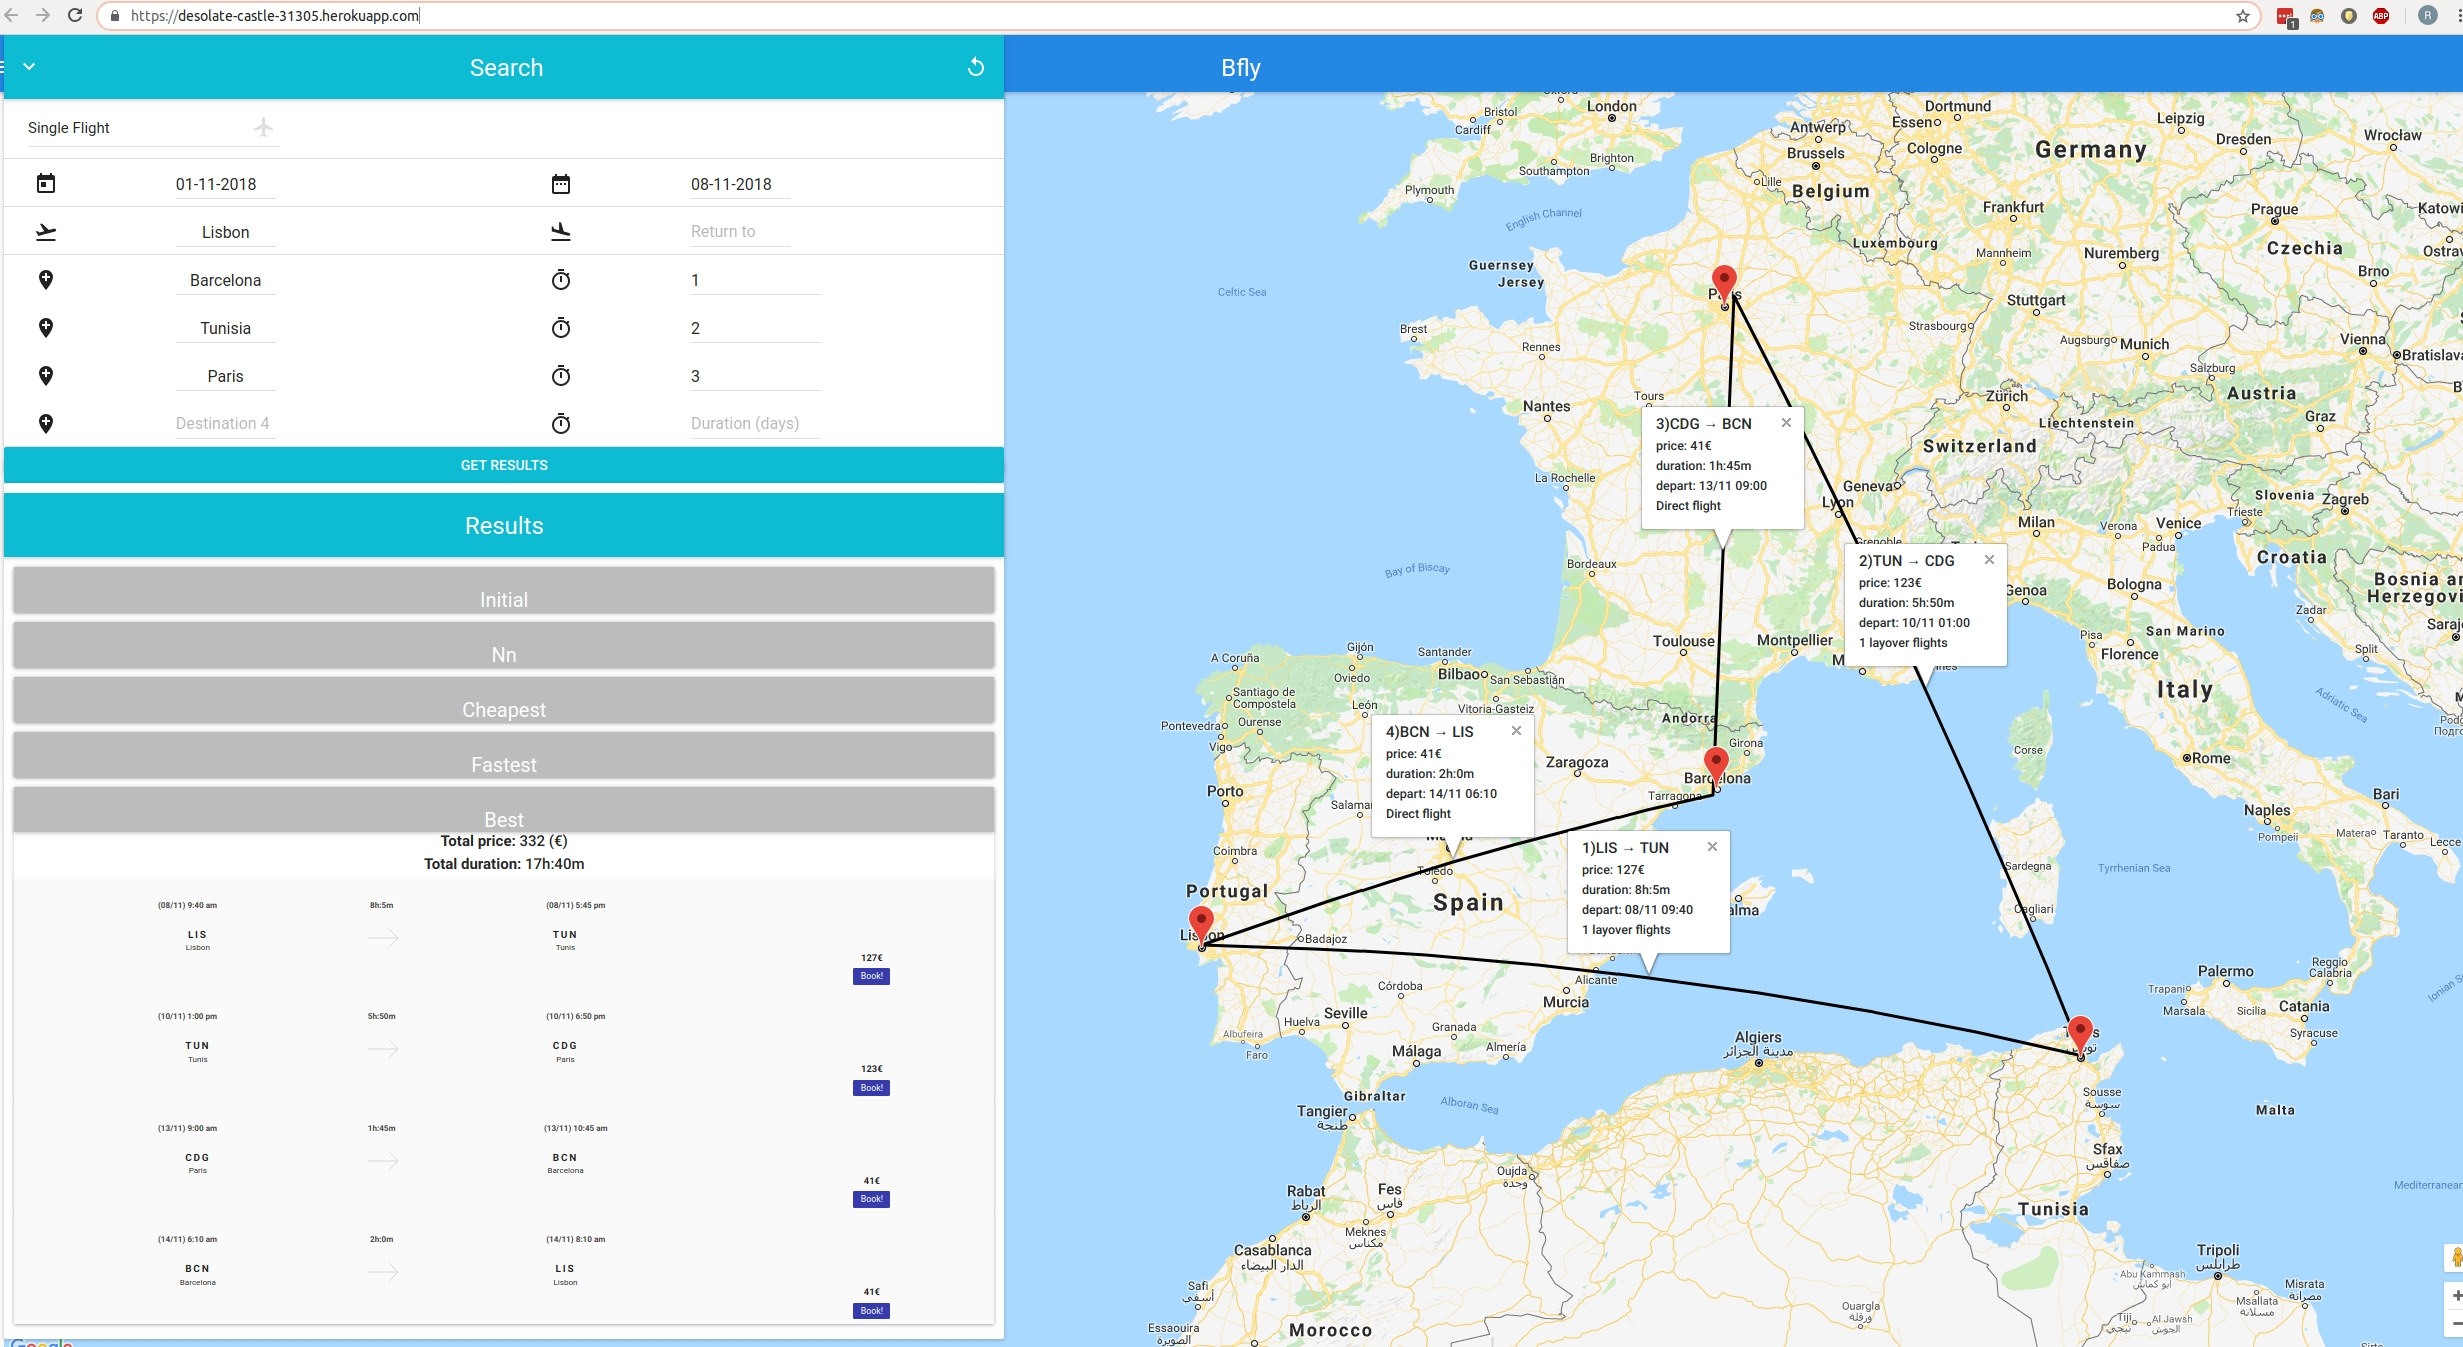
\includegraphics[width=\linewidth]{./imgs/bfly_desktop.jpg}
  \captionof{figure}{Application rendered on desktop.}
 % \caption{Screenshot of the developed application rendered on a desktop device.}
  \label{fig:desktop_app}
\end{minipage}%
\begin{minipage}{.3\textwidth}
  \centering
  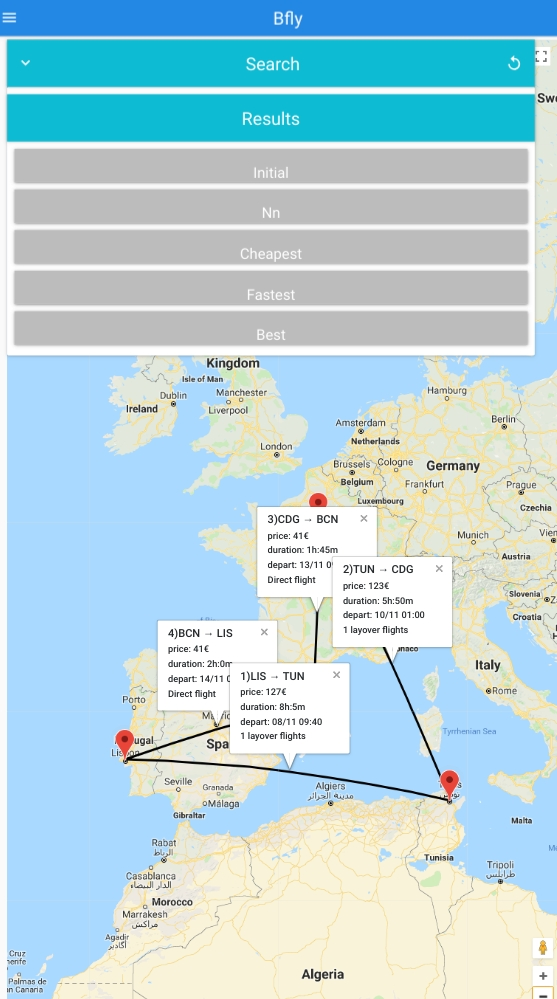
\includegraphics[width=0.75\linewidth]{./imgs/bfly_mobile.jpg}
  \captionof{figure}{Application rended on mobile device.}
  %\caption{Screenshot of the developed application rendered on a mobile device.}
  \label{fig:mobile_app}
\end{minipage}
\end{figure}

